\begin{figure}[ht]
	\centering
	\begin{subfigure}[b]{0.45\textwidth}
		\centering
		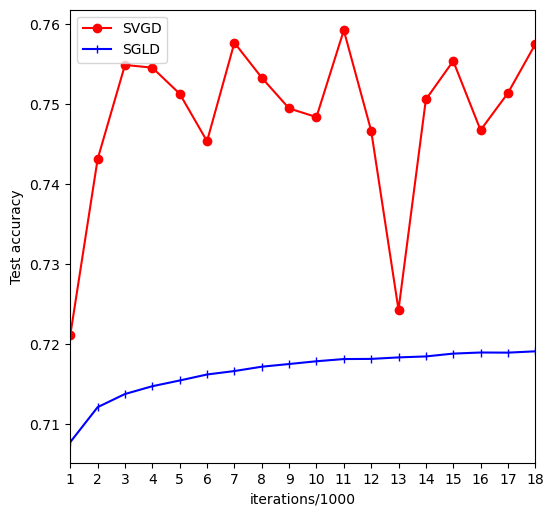
\includegraphics[height=0.2\textheight]{figs/sgvd_sgld_1.png}
		\caption{Test accuracy against every 1000 training iterations}
		\label{fig:acc_iter}
	\end{subfigure}
	\hfill
	\begin{subfigure}[b]{0.45\textwidth}
		\centering
		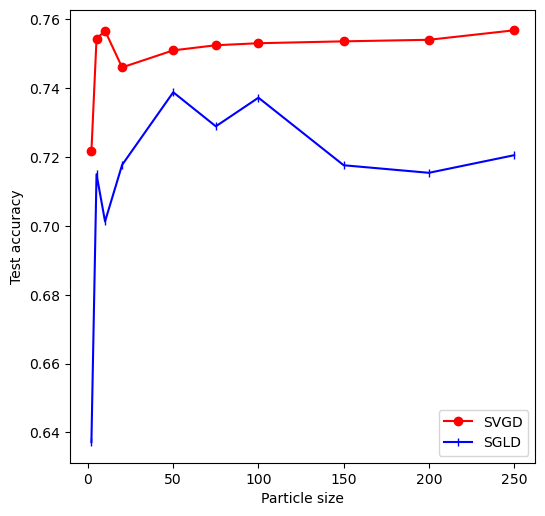
\includegraphics[height=0.2\textheight]{figs/sgvd_sgld_2.png}
		\caption{Test accuracy against number of particles at 3000 iterations ($\frac{1}{3}$ epochs)}
		\label{fig:acc_par}
	\end{subfigure}
	\caption{Results on Bayesian logistic regression on binary Covertype dataset for SVGD and SGLD. Left: Test accuracy against every 1000 training iterations. One epoch is roughly 9000 iterations given the batch size of 50. The number of particles used is 100. Right: Test accuracy against number of particles after 3000 training iterations are done. Experiments are done with 2, 5, 10, 20, 50, 75, 100, 150, 200, 250 particles. The dataset is divided into training and test set with a 8:2 ratio. Each experiment is done on 50 independent trials and the average number is reported.}
	\label{fig:covertype}
\end{figure}